\def\CC{{C\nolinebreak[4]\hspace{-.05em}\raisebox{.4ex}{\tiny\bf ++}}}


\begin{frame}\frametitle{Software development, environment, and testing}
\begin{itemize}
\item E4S: Extreme-Scale Scientific Software Stack % (what, why, how can we use) (1)
\begin{itemize}
\item Pantheon - workflow management
\item DOE Code
\item ECP CI
\end{itemize}
\item IDEAS Team: Better Scientific Software through better practices
% \item Software infrastructure (1)
% \item Case Study: Pantheon (2)
% \item Software process engineering (2)
% \item ECP CI (2)
% \item Are we going to use it? (yes)
% \item DOE Code legacy (1)
\end{itemize}
\end{frame}

\begin{frame}\frametitle{E4S: Extreme-Scale Scientific Software Stack}
Community and infrastructure for developing and deploying software in HPC environments.
\begin{multicols}{2}
\begin{itemize}
\item Heavily spack-based % addresses many issues with conda installer, E4S is the preferred path to contribute to spack
\item Supercontainers (e.g. Docker, Singularity, Shifter)
\item Turnkey environments
\item Standardization of HPC software deployment
\item Collection of build caches
\item ECP stacks, tested, deployed on HPC platforms (ECP CI)
\item Extreme-Scale Scientific Software Development Kits xSDK
\begin{itemize}
\item Math Libraries
\item Data and Visualization
\item Scientific Workflows (Pantheon)
\item Software Ecosystem (DOE Code, ECP CI)
\end{itemize}
%\item Most platforms are already exercising the stacks
%\item Interesting: Can greatly reduce the startup costs of Python due to some cache files not on disk, but in RAM.
%\item Resources, including humans to aid computational science teams with software infrastructure
%\item Policies page
\end{itemize}
\end{multicols}
\begin{center}

\includegraphics[width=.5\textwidth]{figures/e4s.png}\\
https:://e4s-project.github.io
\end{center}
\end{frame}

\begin{frame}\frametitle{E4S for CEESD}
\begin{multicols}{2}
\begin{itemize}
\item Use E4S:
\begin{itemize}
\item \textit{MIRGE} in an E4S turnkey environment
\item Simplify deployment on emerging platforms
\item Accelerate builds and runtime (E4S Build Cache, RAM cache)
\end{itemize}
\columnbreak
%\item Most platforms are already exercising the stacks
%\item Interesting: Can greatly reduce the startup costs of Python due to some cache files not on disk, but in RAM.
\item Join E4S:
\begin{itemize}
\item Requirements (https://e4s-project.github.io/policies.html)
\item Leverage E4S validation test suite (automated deployment!)
\item Resources (a throat to choke)
\item Increased visibility/exposure
\end{itemize}
\end{itemize}
\end{multicols}
\begin{center}

\includegraphics[width=.5\textwidth]{figures/labs.png}\\
https://www.exascaleproject.org/research-project/e4s-and-sdk-efforts/
\end{center}
\end{frame}


%\begin{frame}\frametitle{Software infrastructure}
%\end{frame}

\begin{frame}\frametitle{Pantheon: Reproducible workflows for HPC}
\begin{multicols}{2}
\begin{itemize}
\item What is it?
\begin{itemize}
\item Open standard for workflow specification (https://pantheonscience.org/standards)
%\begin{itemize}
\item YAML-based (install, run, postprocess, validate)
%\end{itemize}
\item What's under-the-covers is your business  (e.g. Parsl, conda)
\item Unification of job design for all supported platforms (includes all lab platforms)
\end{itemize}
\item How can we use it at CEESD?
\begin{itemize}
\item Publish \textit{MIRGE} production workflows
\item Manage/re-imagine multi-platform \textit{MIRGE} performance monitoring/benchmarking
\end{itemize}
\end{itemize}
\end{multicols}
\begin{center}

\includegraphics[width=.2\textwidth]{figures/pantheon.png}\\
https://pantheonscience.org\\
https://github.com/cinemascienceworkflows
\end{center}
\end{frame}

%\begin{frame}\frametitle{ECP - Pantheon - workflow management}
%\begin{itemize}
%\item ``standardizes'' functional description of HPC-oriented workflows
%\item Could most likely use conda
%\item Uses spack closely (integrated)
%\item Maybe replace emirge-like capability with Pantheon
%\item Pantheon use emirge to install and run MIRGE-Com
%\item Integration with parsl?
%\item Re-imagine HPC benchmarking, timings, etc with Pantheon
%\end{itemize}
%\end{frame}

\begin{frame}\frametitle{DOE Code}
\begin{center}
\includegraphics[width=.5\textwidth]{figures/doecode.png}\\
(https://osti.gov/doecode)
\end{center}
\begin{itemize}
\item DOE establishes DOI for the code
\item Maintain/propagate legacy of the DOE-funded code
\item Reduces the big messy pile of DOE-funded code
\item Helps resolve ongoing licensing debacle
\end{itemize}
\end{frame}

\begin{frame}\frametitle{ECP Continuous Integration}
\begin{itemize}
\item CI servers at most major supercomputing sites
\begin{itemize}
\item Operates from site-hosted gitlab instances
\item All currently operating lab-based machines (emerging supported quickly)
\item Regularly exercises ECP codes w/ E4S stacks
\end{itemize}
\item Two ways CEESD could leverage ECP CI:
\begin{itemize}
\item Independent DOE-funded code mirror
\item E4S stack inclusion
\end{itemize}
\end{itemize}
\begin{center}
General ECP-CI Info, documentation: (https://ecp-ci.gitlab.io)\\
LLNL/LC (including Lassen): (https://lc.llnl.gov/gitlab)
\end{center}
\end{frame}

\begin{frame}\frametitle{ECP - IDEAS Team}
\begin{center}
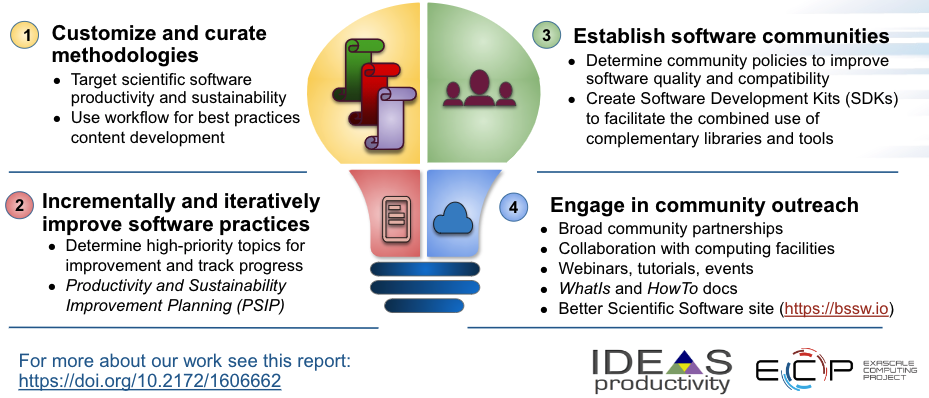
\includegraphics[width=\textwidth]{figures/ideas.png}\\
(https://ideas-productivity.org/ideas-ecp)
\end{center}
\end{frame}

\begin{frame}\frametitle{Software process and practice}\hspace{200pt}
\includegraphics[width=.1\textwidth]{figures/bss.png}
\begin{multicols}{2}
\begin{itemize}
\item Better Scientific Software (https://bssw.io)
\begin{itemize}
\item Best practices - development and project management
\item Training materials and resources
\end{itemize}
\item Some observations questions, and recommendations:
\begin{itemize}
\item Your software will live longer than you expect, so plan for it now (software lifecycle)
\item Consider stand-alone, separate testing suites
\item Restart testing is highly valuable.
\item Resource adaptation is highly valuable.
\item There is a deep interest in performance tracking over time (Kitware supported)
\item Testing tax is mostly imagined.  The cost of defects is extremely high.
\item Onboarding and offboarding procedures are highly valuable.
\end{itemize}
\end{itemize}
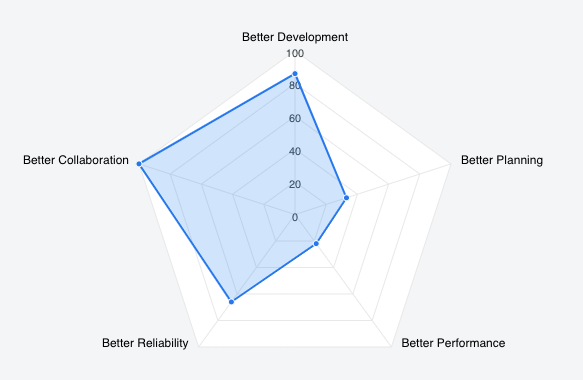
\includegraphics[width=.4\textwidth]{figures/mirge_devel_process_eval.png}
\end{multicols}
\end{frame}



\begin{frame}\frametitle{Better Scientific Software}
\begin{itemize}
\item Improving productivity for users with computing workflows
\item Best practices - for developing and in distributed teams and environments
\item Software practices: Code will live longer than you think (plan now)
\begin{itemize}
\item Testing suites as stand-alone software suites
\item Test-driven development (TDD)
\item Actually test fault detection
\item Focus on exercising your code
\end{itemize}
\item Community guidelines for testing (in-general) needs to be developed:
\begin{itemize}
\item No testing is not enough
\item What is the risk of bugs creeping in?
\item How much time do you spend on defects?
\item How much compute time do you waste computing a spurious result?
\end{itemize}
\item With HPC risk level for defect is very high due to cost of runs
\item Restart tests are highly valuable
\item Code review is highly valuable (think pair coding similar in function, but cost 2x as high)
\item Testing as a part of the development is extremely important
\item Don't forget to test the tests, inject errors on purpose to see if the test catches
\item Small cycles is important - develop test commit test merge test
\item ECP CI is something to help us do CI on the HPC platforms?
\item Deep interest in performance tracking over time - no de-facto standard - so many different angles, so many things that impact performance
\item Interesting: Kitware has taken note, CDash providing native capability for tracking performance over time
\item Test vs. Develop vs. Get work done (testing tax - mostly imagined)
\end{itemize}
\end{frame}

\begin{frame}\frametitle{bof1}
\begin{itemize}
\item build caches of common stacks
\item OS updates underneath can be very costly
\item dependencies work to update is very high
\item Spack based (heavily)
\item Container based (heavily)
\item E4S is the preferred path to contributing to spack
\item ECP projects
\begin{itemize}
\item Vis and analysis
\item tools and building
\item Scientific Workflows 
\end{itemize}
\item e4s-project.github.io/policies.html
\item Supercontainers - containers on the compute platforms
\begin{itemize}
\item Shifter(Cori), singularity(lassen), charliecloud
\item Looks like spack-based build/install can use CI on compute platforms
\item 1. Spock and Articus
\item 2. Make a spack recipe
\item 3. Create smoke tests
\item Support: a throat to choke
\end{itemize}
\end{itemize}
\end{frame}


\begin{frame}\frametitle{bof2}
How to set goals for software improvement?
\begin{itemize}
\item How to measure performance - what metrics
\item performance/dollar
\item performance/watt
\item performance: run faster, don't care how much it costs
\item threshold performance: what performance is required to get done in time
\item relative performance: performance b / performance a
\item IMportant to consider amount of science work done / walltime (accuracy of result inccluded) ECP uses this
\item Identify Figure of Merit (FOM) - that characterizes your performance relative to your end/capstone goal
\item FOM1: \# DOF x \# CG iters / time
\item FOM2: fac1 * \# gp x fac2 * \# part x nsteps / time (facs function of grid push and particle push)
\item Observing high overheads for kernel launch times
\item Parting thoughts:
\begin{itemize}
\item No such thing as *just* porting - refactoring and reprogramming for performance on modern systems touches your code intimately - huge range of different changes
\item Yay for ECP on making it very easy to go from existing CPU code to GPU
\item Totally agree with Point1, disagree Point2 - emphasize teamwork - not a single developer issues - many discussions, many plans
\end{itemize}
\end{itemize}
\end{frame}
% Shot session
% Requirements and <blah> specified by tests is invaluable, highly useful for integration, portability, etc

\begin{frame}\frametitle{Better software}
\begin{itemize}
\item What are your software pain points? (legacy code with no tests)
  - Team turnover
  - Resources to spend on better software (what if you had more funding, what would you spend it on?)
  - Prioritizing science *with the code* over science *into the code* over attention to software process and improvements
    - short time science vs. long-term science : spending on software process and improvements invests in long-term science
  - Reproducibility is a big deal
  - Incorporate these things into your software process, or your code is quickly irrelevant - quickly changing machines, etc
\item What resources do you use to improve your software process?
  - BSSW site
  - Software resource management
\item What would help with your SW development going forward?
\item How could better SW practices reduce risk in your project?
  - Transient developers (team changing in and out) remain useful
\item How do you convince people to improve SW process?
  - How do you convert dug-in skeptics? If you are the skeptic, what would convince you? 
\end{itemize}
\end{frame}

% email watsongr@ornl.gov  about talking about scrum Greg Watson to talk about using Scrum and or other agile software process
% DOE Code - for DOE-funded code, provides DOI for your source
% - instances (closed and public) for DOE codes (GitLab, GitHub, etc)
% - osti.gov
% - code.gov
% - Do not provide access to the code

% Buildtest - schema, yaml - based configurations for get, build, test
% https://github.com/buildtesters/buildtest
% https://buildtest.readthedocs.io/en/latest/what_is_buildtest.html
% Of note: can use buildtest to build and run batched and scheduled tests using a CI-yaml-like configurator 
%  - batch scripts can be written meta
% CDASH is used buildtest_cdash.py

% THursday last session
% https://anl.app.box.com/v/ECP-IC-Annual-Meeting-2021
% e4s.io
% Centralizes the Lab's conversation with the software and hardware vendors
%  - no longer every team doing its own thing with software environments

% ECP VTK-m : many core architectures - No disk I/O required
% Ascent - In Situ viz library
%  - Conduit
%  - funded by ECP Alpine project
% Cinema
%  - github/cinemascience
% VTKm 
% Paraview-Catalyst

% ECP CI
% Can mirror our code to lab-interior gitlab
% Frontier
% Theta: !GPU, general queue
% Iris, Yarrow, Articus
% NERSC: Pretty open, just get account, mirror on their local gitlab (software.nersc.gov)
% Cori: 18 nodes 8 Tesla V100 (haswell, knl, 20xbigmem 2T)
% Ascent system at ORNL: 2xpower9 6 Teslas
% Spock coming - Frontier early access
% Lassen - already has CI runners for batch and bash

% Why does the user care about performance?
% Get the *simulation work* done in time to matter
% Get it done within cost (resource = $$)

% Given a fixed resource, what's the "biggest" simulation that can be done?
% How much faster can the simulation work get done with increased resources?

% Computational resource?
% number of PU * wallclock time

% Simulation work?
% Discrete domain size * simulated time

